\documentclass{article}

\usepackage{graphicx}
\usepackage{tikz}
\usepackage{tikzsymbols}
\usetikzlibrary{calc,patterns,shapes.geometric}
\pagestyle{empty}
\usepackage[margin=0pt]{geometry}
\geometry{papersize={14in,12in}}

\def\centerarc[#1](#2)(#3:#4:#5){\draw[#1] ($(#2)+({#5*cos(#3)},{#5*sin(#3)})$) arc (#3:#4:#5);}

\begin{document}
	\begin{figure}
		\centering
		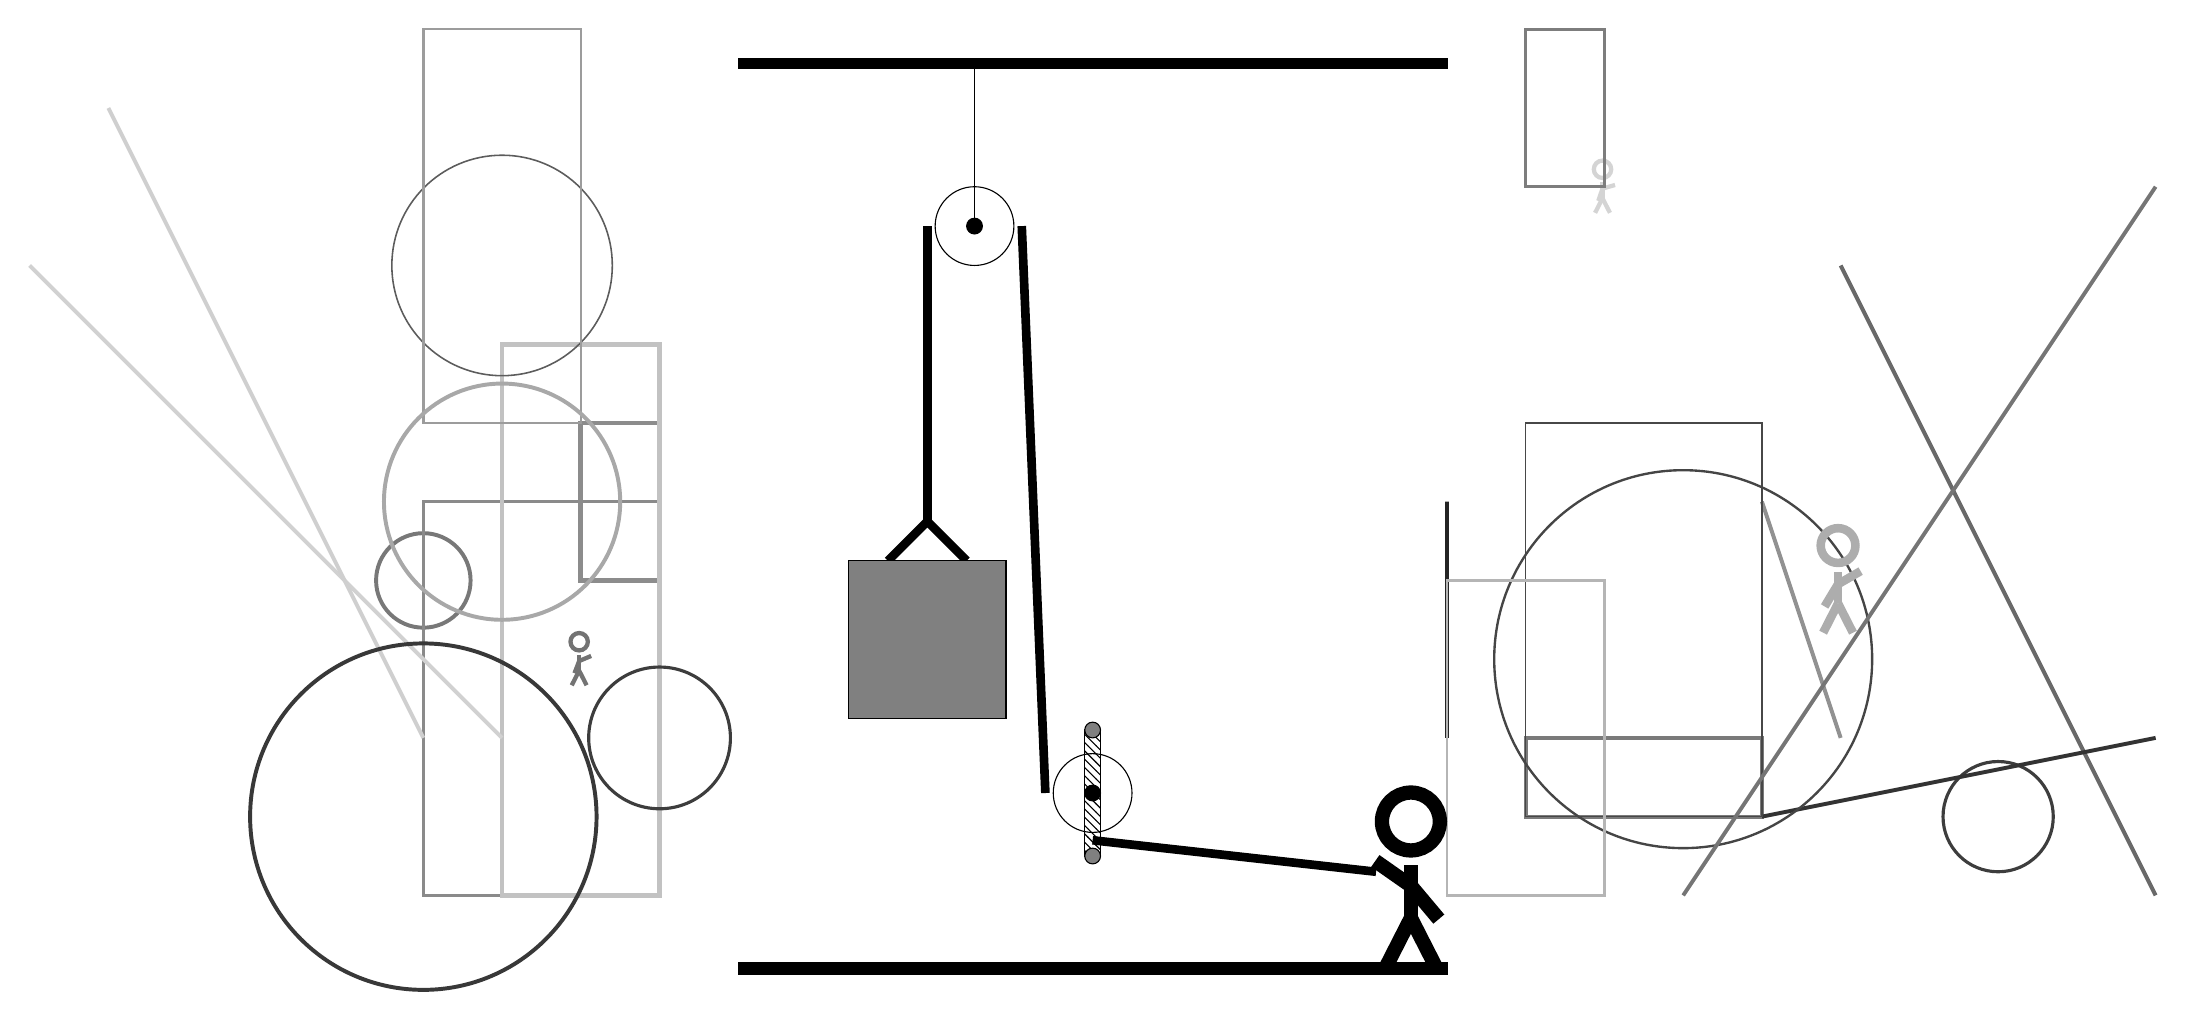
\begin{tikzpicture}
			%%%%% START %%%%%
			
			\draw[fill=black] (-2, 11.5) rectangle (7, 11.625);
			
			\draw[line width=0.5mm, color=black!52] (8, 3) rectangle (11, 2);
			
			\draw [line width=0.5mm, color=black!53](-6, 5) circle (0.6);
			\draw[line width=0.4mm, color=black!46] (-3, 1) rectangle (-6, 6);
			\draw[line width=0.6mm, color=black!45] (-4, 5) rectangle (-3, 7);
			\node[line width=0.5mm, color=black!17] at (9, 10) {\Strichmaxerl[3][71][16]};
			\node[line width=0.2mm, color=black!55] at (-4, 4) {\Strichmaxerl[3][69][23]};
			\draw[line width=0.5mm, color=black!36] (-4, 9) rectangle (-4, 9);
			\draw [line width=0.4mm, color=black!76](14, 2) circle (0.7);
			\draw[line width=0.6mm, color=black!24] (-3, 8) rectangle (-5, 1);
			\draw[line width=0.5mm, color=black!18](-5, 3) -- (-11, 9);
			
			\draw[line width=0.5mm, color=black!59](12, 9) -- (16, 1);
			
			\draw[line width=0.5mm, color=black!43](11, 6) -- (12, 3);
			\draw[line width=0.4mm, color=black!86] (7, 3) rectangle (7, 6);
			
			\draw[line width=0.5mm, color=black!19](-6, 3) -- (-10, 11);
			\draw[line width=0.5mm, color=black!80](11, 2) -- (16, 3);
			\draw[line width=0.4mm, color=black!51] (9, 10) rectangle (8, 12);
			
			\draw [line width=0.2mm, color=black!64](-5, 9) circle (1.4);
			
			\draw[line width=0.3mm, color=black!39] (-4, 12) rectangle (-6, 7);
			\draw [line width=0.5mm, color=black!78](-6, 2) circle (2.2);
			
			\draw[line width=0.2mm, color=black!72] (8, 7) rectangle (11, 2);
			\draw [line width=0.3mm, color=black!73](10, 4) circle (2.4);
			
			\draw [line width=0.4mm, color=black!76](-3, 3) circle (0.9);
			\draw[line width=0.3mm, color=black!29] (7, 1) rectangle (9, 5);
			\draw[line width=0.5mm, color=black!54](10, 1) -- (16, 10);
			\draw [line width=0.5mm, color=black!34](-5, 6) circle (1.5);
			\node[line width=0.4mm, color=black!32] at (12, 5) {\Strichmaxerl[6][59][30]};
			
			\draw (1, 9.5) circle (0.5);
			\draw[fill=black] (1, 9.5) circle (0.1);
			\draw (1, 11.5) -- (1, 9.5);
			
			\draw[fill=white](2.5, 2.3) circle (0.5);
			\draw[fill=black] (2.5, 2.3) circle (0.1);
			\draw[pattern=north west lines, pattern color=black] (2.4, 3.1) rectangle (2.6, 1.5);
			\draw[fill=black!50] (2.5, 3.1) circle (0.1);
			\draw[fill=black!50] (2.5, 1.5) circle (0.1);
			
			\draw[line width=1.1mm] (-0.1, 5.25) -- (0.4, 5.75) -- (0.9, 5.25);
			\draw[fill=black!50] (-0.6, 5.25) rectangle (1.4, 3.25);
			
			\draw[line width=1.1mm] (0.4, 9.5) -- (0.4, 5.75);
			\centerarc[line width=1.1mm](1, 9.5)(0:180:0.6);
			\draw[line width=1.1mm](1.6, 9.5) -- (1.9, 2.3);
			\centerarc[line width=1.1mm](2.5, 2.3)(180:270:0.6);
			\draw[line width=1.1mm](2.5, 1.7) -- (6.1, 1.3);
			
			\node at (6.5, 1.2) {\Strichmaxerl[10][-35][-50]};
			
			\draw[fill=black] (-2, 0) rectangle (7, 0.15);
			
			%%%%% END %%%%%
		\end{tikzpicture}
	\end{figure}	
\end{document}